\documentclass[letterpaper, 12pt]{article}
\usepackage[letterpaper, top=2.5cm, bottom=2.5cm, left=3cm, right=3cm]{geometry} %margenes
\usepackage[utf8]{inputenc} %manejo de caracteres especiales
\usepackage[spanish]{babel} %manejo de encabezados de inglés a español
\usepackage{fancyhdr} %formato de los encabezados de página
\usepackage{ragged2e} %alineado real justficado
\usepackage{graphicx} %manejo de imagenes
\usepackage{amsmath} %manejo de notación matemática
\usepackage{mathtools} %manejo de notación matemática
\usepackage{blindtext} %texto de relleno
\usepackage{cancel} %permite la simbolización de cancelación de terminos
\usepackage{enumitem}[shortlabels] %listas con letras
\usepackage{amssymb} %manejo de simbología matematica
\usepackage{float}

\pagestyle{fancy}
\fancyhf{}
\rfoot{}

\begin{document}
\thispagestyle{fancy}
\lhead{\textbf{Nombre: Abraham Jhared Flores Azcona\\\#: 19211640}}
\rhead{\textbf{Actividad 6\\Parte 2}}
\section*{Newton-Raphson}
\subsection*{Elabora un resumen de lo explicado en el 2do video adjunto a la actividad de Classroom con procedimientos y fórmulas}
\justify
A grandes rasgos, este método para encontrar raíces de una función recae en el uso de la interpretación geométrica de la derivada. 
\\\newline
Para todo método iterativo para calcular raices, se quiere llegar a la coordenada \((x_r,0)\) donde \(x_r\) corresponde al valor de 
\(x\) de la raíz y el cero presente en el lugar de \(y\) es debido a que una raíz de una función hace entender que
esta ``en medio'' del eje de las abcisas, que hace entender que no tenga algún tipo de ascenso con respecto a \(y\), por ende la referencia a una raíz.
\\\newline
Primero se elige un valor inicial de \(x\) cualquiera para empezar el procedimiento, se traza una linea recta perdendicular al eje \(y\) desde la
coordenada del valor elejido de \(x\) (llamese \(x_i\)) y la intersección que dicha recta haga con la función será la coordenada \((x_i,f(x_i))\).
\begin{figure}[H]
    \centering
    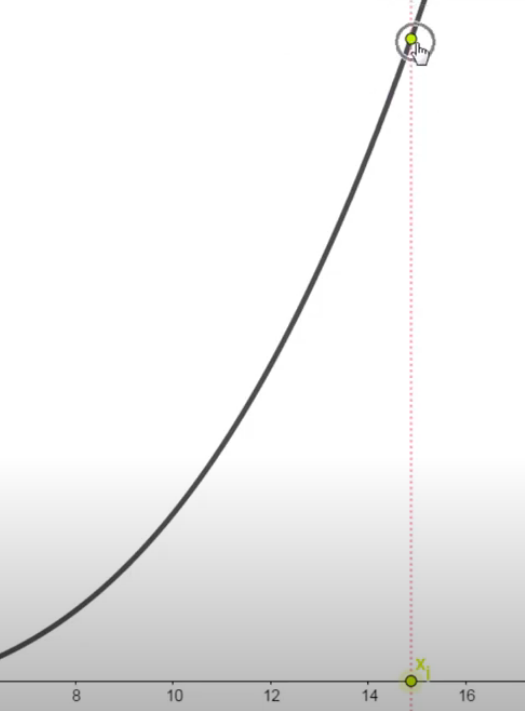
\includegraphics[height=5.5cm,width=6cm]{primero.PNG}
\end{figure}
\justify
Despues en \(x_i,f(x_i)\) se traza una recta tangente a la gráfica, y en el punto donde esta recta tangente intersecta al eje de las abcisas, se realiza otra vez el proceso
hasta llegar a la raíz, o hasta realizar cierta cantidad de iteraciones.
\begin{figure}[H]
    \centering
    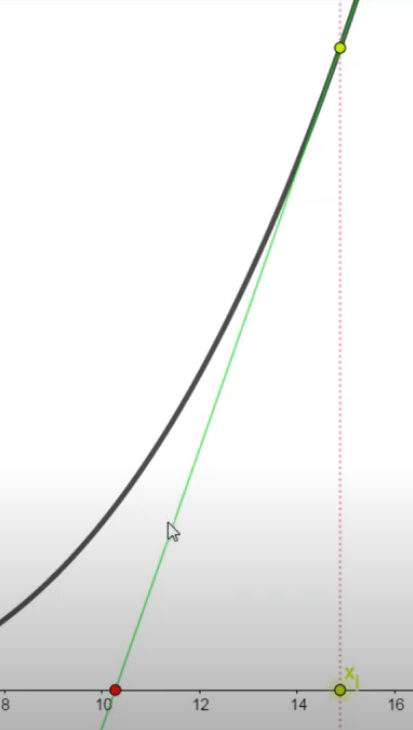
\includegraphics[height=5.5cm,width=6cm]{Despues.PNG}
\end{figure}
\justify
Expresado de manera matemática, como se habla de rectas, empezamos usando la fórmula de una recta:
\[y-y_1=m(x-x_1)\]
Cambiando los índices de las variables para acomodar a lo estipulado antes:
\[y-y_i=m(x-x_i)\]
Considerando que la gráfica es una función, entonces \(y=f(x)\) y por ello:
\[y-y_i=m(x-x_i)\rightarrow f(x)-f(x_i)=m(x-x_i)\]
En este caso, como esta recta se considera como tangente a la gráfica por el proceso, sabemos que su pendiente es la derivada de la función:
\[f(x)-f(x_i)=f^{\prime}\!(x_i)(x-x_i)\]
Como estamos calculando raíces, se sobreentiende que la coordenada de una raíz tiene la forma \((x,0)\), por ello:
\[f(x)-f(x_i)=f^{\prime}\!(x_i)(x-x_i)\rightarrow -f(x_i)=f^{\prime}\!(x_i)(x-x_i)\]
Despejamos para \(x\):
\begin{equation*}
    \begin{aligned}
        -f(x_i)&=f^{\prime}\!(x_i)(x-x_i)\\[5pt]
        -\frac{f(x_i)}{f^{\prime}\!(x_i)}&=x-x_i\\[5pt]
        x_i-\frac{f(x_i)}{f^{\prime}\!(x_i)}&=x\\[5pt]
        x&=x_i-\frac{f(x_i)}{f^{\prime}\!(x_i)}\\[5pt]
    \end{aligned}
\end{equation*}
Finalmente, como el método de Newton-Raphson es iterativo, se comprende que el valor de \(x\) va a ser el siguiente de \(x_i\), por lo que \(x\rightarrow x_{i+1}\):
\[x_{i+1}=x_i-\frac{f(x_i)}{f^{\prime}\!(x_i)}\]
\end{document}